% Options for packages loaded elsewhere
\PassOptionsToPackage{unicode}{hyperref}
\PassOptionsToPackage{hyphens}{url}
%
\documentclass[
  letterpaper,
  ignorenonframetext,
  aspectratio=43,
  handout,
  12pt]{beamer}
\usepackage{pgfpages}
\setbeamertemplate{caption}[numbered]
\setbeamertemplate{caption label separator}{: }
\setbeamercolor{caption name}{fg=normal text.fg}
\beamertemplatenavigationsymbolsempty
% Prevent slide breaks in the middle of a paragraph
\widowpenalties 1 10000
\raggedbottom
\setbeamertemplate{part page}{
  \centering
  \begin{beamercolorbox}[sep=16pt,center]{part title}
    \usebeamerfont{part title}\insertpart\par
  \end{beamercolorbox}
}
\setbeamertemplate{section page}{
  \centering
  \begin{beamercolorbox}[sep=12pt,center]{part title}
    \usebeamerfont{section title}\insertsection\par
  \end{beamercolorbox}
}
\setbeamertemplate{subsection page}{
  \centering
  \begin{beamercolorbox}[sep=8pt,center]{part title}
    \usebeamerfont{subsection title}\insertsubsection\par
  \end{beamercolorbox}
}
\AtBeginPart{
  \frame{\partpage}
}
\AtBeginSection{
  \ifbibliography
  \else
    \frame{\sectionpage}
  \fi
}
\AtBeginSubsection{
  \frame{\subsectionpage}
}
\usepackage{amsmath,amssymb}
\usepackage{lmodern}
\usepackage{iftex}
\ifPDFTeX
  \usepackage[T1]{fontenc}
  \usepackage[utf8]{inputenc}
  \usepackage{textcomp} % provide euro and other symbols
\else % if luatex or xetex
  \usepackage{unicode-math}
  \defaultfontfeatures{Scale=MatchLowercase}
  \defaultfontfeatures[\rmfamily]{Ligatures=TeX,Scale=1}
\fi
\usetheme[]{metropolis}
% Use upquote if available, for straight quotes in verbatim environments
\IfFileExists{upquote.sty}{\usepackage{upquote}}{}
\IfFileExists{microtype.sty}{% use microtype if available
  \usepackage[]{microtype}
  \UseMicrotypeSet[protrusion]{basicmath} % disable protrusion for tt fonts
}{}
\makeatletter
\@ifundefined{KOMAClassName}{% if non-KOMA class
  \IfFileExists{parskip.sty}{%
    \usepackage{parskip}
  }{% else
    \setlength{\parindent}{0pt}
    \setlength{\parskip}{6pt plus 2pt minus 1pt}}
}{% if KOMA class
  \KOMAoptions{parskip=half}}
\makeatother
\usepackage{xcolor}
\IfFileExists{xurl.sty}{\usepackage{xurl}}{} % add URL line breaks if available
\IfFileExists{bookmark.sty}{\usepackage{bookmark}}{\usepackage{hyperref}}
\hypersetup{
  hidelinks,
  pdfcreator={LaTeX via pandoc}}
\urlstyle{same} % disable monospaced font for URLs
\newif\ifbibliography
\usepackage{longtable,booktabs,array}
\usepackage{calc} % for calculating minipage widths
\usepackage{caption}
% Make caption package work with longtable
\makeatletter
\def\fnum@table{\tablename~\thetable}
\makeatother
\usepackage{graphicx}
\makeatletter
\def\maxwidth{\ifdim\Gin@nat@width>\linewidth\linewidth\else\Gin@nat@width\fi}
\def\maxheight{\ifdim\Gin@nat@height>\textheight\textheight\else\Gin@nat@height\fi}
\makeatother
% Scale images if necessary, so that they will not overflow the page
% margins by default, and it is still possible to overwrite the defaults
% using explicit options in \includegraphics[width, height, ...]{}
\setkeys{Gin}{width=\maxwidth,height=\maxheight,keepaspectratio}
% Set default figure placement to htbp
\makeatletter
\def\fps@figure{htbp}
\makeatother
% Make links footnotes instead of hotlinks:
\DeclareRobustCommand{\href}[2]{#2\footnote{\url{#1}}}
\setlength{\emergencystretch}{3em} % prevent overfull lines
\providecommand{\tightlist}{%
  \setlength{\itemsep}{0pt}\setlength{\parskip}{0pt}}
\setcounter{secnumdepth}{-\maxdimen} % remove section numbering
\usepackage{pgfpages}
\pgfpagesuselayout{2 on 1}
\providecommand{\tightlist}{%
\setlength{\itemsep}{0pt}\setlength{\parskip}{0pt}}
\makeatletter
\makeatother
\let\Oldincludegraphics\includegraphics
\renewcommand{\includegraphics}[2][]{\Oldincludegraphics[width=\textwidth,height=0.7\textheight,keepaspectratio]{#2}}
\ifLuaTeX
  \usepackage{selnolig}  % disable illegal ligatures
\fi

\author{}
\date{}

\begin{document}

\begin{frame}{Theory of Elasticity}
\protect\hypertarget{theory-of-elasticity}{}
Dr.~Nicholas Smith

Wichita State University, Department of Aerospace Engineering October
21, 2021
\end{frame}

\begin{frame}{upcoming schedule}
\protect\hypertarget{upcoming-schedule}{}
\begin{itemize}
\tightlist
\item
  Oct 21 - Airy Stress Functions
\item
  Oct 22 - Homework 5 Self-Grade Due
\item
  Oct 26 - SPTE, Airy Stress
\item
  Oct 28 - Airy Stress
\item
  Oct 29 - Homework 6 Due
\item
  Nov 2 - Airy Stress
\end{itemize}
\end{frame}

\begin{frame}{outline}
\protect\hypertarget{outline}{}
\begin{itemize}
\tightlist
\item
  two-dimensional problems
\item
  plane strain
\item
  plane stress
\item
  generalized plane stress
\end{itemize}
\end{frame}

\hypertarget{two-dimensional-problems}{%
\section{two-dimensional problems}\label{two-dimensional-problems}}

\begin{frame}{2d problems}
\protect\hypertarget{d-problems}{}
\begin{itemize}
\tightlist
\item
  As we learned in Chapter 5, it is often very difficult to solve full
  problems in 3D
\item
  Some problems contain symmetry, or particular geometries which allow
  certain simplifications to be made
\item
  In this chapter we will consider the following 2D formulations

  \begin{itemize}
  \tightlist
  \item
    Plane strain
  \item
    Plane stress
  \item
    Generalized plane stress
  \item
    Antiplane strain
  \end{itemize}
\end{itemize}
\end{frame}

\begin{frame}{2d problems}
\protect\hypertarget{d-problems-1}{}
\begin{itemize}
\tightlist
\item
  Airy stress functions provide a systematic method for solving 2D
  problems
\item
  We will also develop Airy stress function solution methods in polar
  (cylindrical or spherical) coordinates
\end{itemize}
\end{frame}

\hypertarget{plane-strain}{%
\section{plane strain}\label{plane-strain}}

\begin{frame}{plane strain}
\protect\hypertarget{plane-strain-1}{}
\begin{itemize}
\tightlist
\item
  Plane strain is a state we consider for very long bodies
\item
  If the body is sufficiently long, then the deformation field can be
  considered to be a function of \emph{x} and \emph{y} only
\end{itemize}

\[\begin{aligned}
    u &= u(x,y)\\
    v &= v(x,y)\\
    w &= 0
\end{aligned}\]
\end{frame}

\begin{frame}{plane strain}
\protect\hypertarget{plane-strain-2}{}
\begin{itemize}
\tightlist
\item
  We can use the strain-displacement relations to find the corresponding
  strains from our assumptions on the displacement
\end{itemize}

\[\begin{aligned}
    \epsilon_{xx} &= \frac{\partial u}{\partial x}\\
    \epsilon_{yy} &= \frac{\partial v}{\partial y}\\
    \epsilon_{xy} &= \frac{1}{2}\left(\frac{\partial u}{\partial y} + \frac{\partial v}{\partial x}\right)\\
    \epsilon_{zz} &= \epsilon_{xz} = \epsilon_{yz} = 0
\end{aligned}\]
\end{frame}

\begin{frame}{plane strain}
\protect\hypertarget{plane-strain-3}{}
\begin{itemize}
\tightlist
\item
  We can use Hooke's law to find the stresses
\end{itemize}

\[\begin{aligned}
    \sigma_{xx} &= \lambda(\epsilon_{xx} + \epsilon_{yy}) + 2\mu \epsilon_{xx}\\
    \sigma_{yy} &= \lambda(\epsilon_{xx} + \epsilon_{yy}) + 2\mu \epsilon_{yy}\\
    \sigma_{zz} &= \lambda(\epsilon_{xx} + \epsilon_{yy})\\
    \tau_{xy} &= 2\mu \epsilon_{xy} \\
    \tau_{xz} &= \tau_{yz} = 0
\end{aligned}\]
\end{frame}

\begin{frame}{plane strain}
\protect\hypertarget{plane-strain-4}{}
\begin{itemize}
\tightlist
\item
  We can use these relationships to reduce the equilibrium equations.
\item
  Recall that for equilibrium we have
\end{itemize}

\[\sigma_{ij,j} + F_i = 0\]

\[\tau_{xz} = \tau_{yz} = 0\], so those terms will vanish
\end{frame}

\begin{frame}{plane strain}
\protect\hypertarget{plane-strain-5}{}
\begin{itemize}
\tightlist
\item
  Although \(\sigma_{zz} \ne 0\), it only appears with a derivative of
  \emph{z}, and it is a function of \emph{x} and \emph{y} only, so
  \(\sigma_{zz}\) will not appear in any non-trivial equilibrium
  equation
\end{itemize}

\[\begin{aligned}
    \frac{\partial \sigma_{xx}}{\partial x} + \frac{\partial \tau_{xy}}{\partial y} + F_x &= 0\\
    \frac{\partial \tau_{xy}}{\partial x} +\frac{\partial \sigma_{yy}}{\partial y} +  F_y &= 0
\end{aligned}\]
\end{frame}

\begin{frame}{plane strain}
\protect\hypertarget{plane-strain-6}{}
\begin{itemize}
\tightlist
\item
  We can use the strain-displacement equations and Hooke's Law to write
  Navier's equations for plane strain
\end{itemize}

\[\begin{aligned}
    \mu \nabla^2 u + (\lambda + \mu) \frac{\partial}{\partial x} \left(\frac{\partial u}{\partial x} + \frac{\partial v}{\partial y}\right) + F_x &= 0\\
    \mu \nabla^2 v + (\lambda + \mu) \frac{\partial}{\partial y} \left(\frac{\partial u}{\partial x} + \frac{\partial v}{\partial y}\right) + F_x &= 0
\end{aligned}\]
\end{frame}

\begin{frame}{compatibility}
\protect\hypertarget{compatibility}{}
\[\begin{aligned}
    \frac{\partial^2 \epsilon_x}{\partial y^2} + \frac{\partial^2 \epsilon_y}{\partial x^2} &= 2\frac{\partial^2 \epsilon_{xy}}{\partial x \partial y}\\
    \frac{\partial^2 \epsilon_y}{\partial z^2} + \frac{\partial^2 \epsilon_z}{\partial y^2} &= 2\frac{\partial^2 \epsilon_{yz}}{\partial y \partial z}\\
    \frac{\partial^2 \epsilon_z}{\partial x^2} + \frac{\partial^2 \epsilon_x}{\partial z^2} &= 2\frac{\partial^2 \epsilon_{zx}}{\partial z \partial x}\\
    \frac{\partial^2 \epsilon_x}{\partial y \partial z} &= \frac{\partial}{\partial x} \left(-\frac{\partial \epsilon_{yz}}{\partial x} + \frac{\partial \epsilon_{zx}}{\partial y} + \frac{\partial \epsilon_{xy}}{\partial z}\right)\\
    \frac{\partial^2 \epsilon_y}{\partial z \partial x} &= \frac{\partial}{\partial y} \left(-\frac{\partial \epsilon_{zx}}{\partial y} + \frac{\partial \epsilon_{xy}}{\partial z} + \frac{\partial \epsilon_{yz}}{\partial x}\right)\\
    \frac{\partial^2 \epsilon_z}{\partial x \partial y} &= \frac{\partial}{\partial z} \left(-\frac{\partial \epsilon_{xy}}{\partial z} + \frac{\partial \epsilon_{yz}}{\partial x} + \frac{\partial \epsilon_{zx}}{\partial y}\right)
\end{aligned}\]
\end{frame}

\begin{frame}{plane strain}
\protect\hypertarget{plane-strain-7}{}
\begin{itemize}
\tightlist
\item
  The only non-trivial term from the compatibility equations is
\end{itemize}

\[\frac{\partial^2 \epsilon_x}{\partial y^2} + \frac{\partial^2 \epsilon_y}{\partial x^2} = 2\frac{\partial^2 \epsilon_{xy}}{\partial x \partial y}\]

\begin{itemize}
\tightlist
\item
  This can also be written in terms of stress (Beltrami-Mitchell)
\end{itemize}

\[\nabla^2(\sigma_x + \sigma_y) = -\frac{1}{1-\nu}\left(\frac{\partial F_x}{\partial x} + \frac{\partial F_y}{\partial y}\right)\]
\end{frame}

\begin{frame}{plane strain}
\protect\hypertarget{plane-strain-8}{}
\begin{itemize}
\tightlist
\item
  Plane strain is exact for a body of infinite length, but can also be
  useful for real shapes of finite length
\item
  Consider a long body with fixed and frictionless ends.
\item
  The boundary conditions for this case are
\end{itemize}

\[\begin{aligned}
    w(x,y,\pm L) &= 0\\
    \tau_{xz}(x,y,\pm L) &= 0\\
    \tau_{yz}(x,y,\pm L) &= 0
\end{aligned}\]
\end{frame}

\hypertarget{plane-stress}{%
\section{plane stress}\label{plane-stress}}

\begin{frame}{plane stress}
\protect\hypertarget{plane-stress-1}{}
\begin{itemize}
\tightlist
\item
  If the thickness of a body is small compared to the other dimensions,
  we assume that there can not be much variation in any of the stress
  components in that direction
\item
  The assumptions for plane stress can be summarized as
\end{itemize}

\[\begin{aligned}
    \sigma_x &= \sigma_x(x,y)\\
    \sigma_y &= \sigma_y(x,y)\\
    \tau_{xy} &= \tau_{xy}(x,y)\\
    \sigma_z &= \tau_{xz} = \tau_{yz} = 0
\end{aligned}\]
\end{frame}

\begin{frame}{plane stress}
\protect\hypertarget{plane-stress-2}{}
\begin{itemize}
\tightlist
\item
  To maintain these assumptions, there can be no body forces in the
  \emph{z}-direction and no applied tractions in the \emph{z}-direction.
\item
  Other body forces must be independent of \emph{z}, or distributed
  symmetrically such that the average may be used.
\end{itemize}
\end{frame}

\begin{frame}{plane stress}
\protect\hypertarget{plane-stress-3}{}
\begin{itemize}
\tightlist
\item
  We can use Hooke's law to find the corresponding values of strain
\end{itemize}

\[\begin{aligned}
    \epsilon_x &= \frac{1}{E}(\sigma_x - \nu \sigma_y)\\
    \epsilon_y &= \frac{1}{E}(\sigma_y - \nu \sigma_x)\\
    \epsilon_z &= -\frac{\nu}{E}(\sigma_x + \sigma_y)\\
    \epsilon_{xy} &= \frac{1+\nu}{E}\tau_{xy}\\
    \epsilon_{xz} &= \epsilon_{yz} = 0
\end{aligned}\]
\end{frame}

\begin{frame}{strain-displacement}
\protect\hypertarget{strain-displacement}{}
\[\begin{aligned}
    \epsilon_{x} &= \frac{\partial u}{\partial x}\\
    \epsilon_{y} &= \frac{\partial v}{\partial y}\\
    \epsilon_{z} &= \frac{\partial w}{\partial z}\\
    \epsilon_{xy} &= \frac{1}{2}\left(\frac{\partial u}{\partial y} + \frac{\partial v}{\partial x}\right)\\
    \epsilon_{yz} &= \frac{1}{2}\left(\frac{\partial v}{\partial z} + \frac{\partial w}{\partial y}\right) = 0\\
    \epsilon_{xz} &= \frac{1}{2}\left(\frac{\partial u}{\partial z} + \frac{\partial w}{\partial x}\right) = 0\\
\end{aligned}\]
\end{frame}

\begin{frame}{plane stress}
\protect\hypertarget{plane-stress-4}{}
\begin{itemize}
\tightlist
\item
  Since strain in the \emph{z}-direction is not zero, \emph{w} becomes a
  linear function of \emph{z}
\item
  We also find that \emph{u} and \emph{v} will also be functions of
  \emph{z}
\item
  These effects are normally neglected, leading to an approximation in
  the formulation
\item
  This is why we cannot use the full 3D compatibility equations to
  assess compatibility of a body with an assumed state of plane stress
\end{itemize}
\end{frame}

\begin{frame}{plane stress}
\protect\hypertarget{plane-stress-5}{}
\begin{itemize}
\tightlist
\item
  The equilibrium equations reduce the same form in plane stress as they
  did for plane strain
\end{itemize}

\[\begin{aligned}
    \frac{\partial \sigma_{xx}}{\partial x} + \frac{\partial \tau_{xy}}{\partial y} + F_x &= 0\\
    \frac{\partial \tau_{xy}}{\partial x} +\frac{\partial \sigma_{yy}}{\partial y} +  F_y &= 0
\end{aligned}\]

\begin{itemize}
\tightlist
\item
  But the Navier equations in terms of displacement do not reduce to
  exactly the same form
\end{itemize}

\[\begin{aligned}
    \mu \nabla^2 u + \frac{E}{2(1-\nu)} \frac{\partial}{\partial x} \left(\frac{\partial u}{\partial x} + \frac{\partial v}{\partial y}\right) + F_x &= 0\\
    \mu \nabla^2 v + \frac{E}{2(1-\nu)} \frac{\partial}{\partial y} \left(\frac{\partial u}{\partial x} + \frac{\partial v}{\partial y}\right) + F_y &= 0
\end{aligned}\]
\end{frame}

\begin{frame}{navier equations}
\protect\hypertarget{navier-equations}{}
\begin{itemize}
\tightlist
\item
  The factor in the plane strain Navier equations is
\end{itemize}

\[(\lambda + \mu)\]

\begin{itemize}
\tightlist
\item
  We can convert this to \(E\), \(\nu\) to better compare with the plane
  stress equation
\end{itemize}
\end{frame}

\begin{frame}{navier equations}
\protect\hypertarget{navier-equations-1}{}
\[\begin{aligned}
    \lambda + \mu &= \frac{\nu E}{(1+\nu)(1-2\nu)} + \frac{E}{2(1+\nu)}\\
    &= \frac{2\nu E}{2(1+\nu)(1-2\nu)} + \frac{E(1-2\nu)}{2(1+\nu)(1-2\nu)}\\
    &= \frac{2\nu E + E - 2\nu E}{2(1+\nu)(1-2\nu)}\\
    &= \frac{E}{2(1+\nu)(1-2\nu)}
\end{aligned}\]
\end{frame}

\begin{frame}{compatibility}
\protect\hypertarget{compatibility-1}{}
\begin{itemize}
\tightlist
\item
  Due to the approximations we made earlier, we neglect all
  compatibility equations with \(\epsilon_z\), even though these may not
  be zero
\end{itemize}

\[\frac{\partial^2 \epsilon_x}{\partial y^2} + \frac{\partial^2 \epsilon_y}{\partial x^2} = 2 \frac{\partial^2 \epsilon_{xy}}{\partial x \partial y}\]

\begin{itemize}
\tightlist
\item
  or in terms of stress
\end{itemize}

\[\nabla^2 (\sigma_{xx} + \sigma_{yy}) = -(1+\nu)\left(\frac{\partial F_x}{\partial x} + \frac{\partial F_y}{\partial y}\right)\]
\end{frame}

\begin{frame}{conversion}
\protect\hypertarget{conversion}{}
\begin{itemize}
\tightlist
\item
  While plane strain and plane stress give similar results, they are not
  identical
\item
  We can convert between plane strain and plane stress by replacing
  \emph{E} and \(\nu\)
\end{itemize}

\begin{longtable}[]{@{}ccc@{}}
\toprule
& \emph{E} & \(\nu\) \\
\midrule
\endhead
Plane stress to plane strain & \(\frac{E}{1-\nu^2}\) &
\(\frac{v}{1-\nu}\) \\
Plane strain to plane stress & \(\frac{E(1+2\nu)}{1+\nu^2}\) &
\(\frac{v}{1+\nu}\) \\
\bottomrule
\end{longtable}

\begin{itemize}
\tightlist
\item
  When \(\nu = 0\), plane strain and plane stress give identical results
\end{itemize}
\end{frame}

\hypertarget{generalized-plane-stress}{%
\section{generalized plane stress}\label{generalized-plane-stress}}

\begin{frame}{generalized plane stress}
\protect\hypertarget{generalized-plane-stress-1}{}
\begin{itemize}
\tightlist
\item
  Some approximations introduced inconsistencies in the plane stress
  formulation
\item
  Generalized plane stress is based on averaging the field quantities
  through the thickness
\end{itemize}

\[\bar{\psi} = \frac{1}{2h} \int_{-h}^{h}\psi (x,y,z) dz\]
\end{frame}

\begin{frame}{generalized}
\protect\hypertarget{generalized}{}
\begin{itemize}
\tightlist
\item
  We again assume that the thickness, \(2h\), is much smaller than the
  other dimensions
\item
  We also assume that tractions on the surfaces \(z = \pm h\) are zero
\item
  Edge loadings must have no \emph{z} component and are independent of
  \emph{z}
\item
  Body forces also cannot have a \emph{z} component and must be
  independent of \emph{z} or symmetrically distributed through the
  thickness
\item
  This gives \emph{w} as a linear function of \emph{z} which means
\end{itemize}

\[w(x,y,z) = -w(x,y,-z)\]
\end{frame}

\begin{frame}{average field variables}
\protect\hypertarget{average-field-variables}{}
\[\begin{aligned}
    \bar{u} &= \bar{u}(x,y)\\
    \bar{v} &= \bar{v}(x,y)\\
    \bar{w} &= \bar{w}(x,y)\\
    \bar{\sigma_z} &= \bar{\tau_{xz}} = \bar{\tau_{yz}} = 0\\
    \bar{\sigma_x} &= \lambda^\*(\bar{\epsilon_x}+\bar{\epsilon_y}) + 2\mu \bar{\epsilon_x}\\
    \bar{\sigma_y} &= \lambda^\*(\bar{\epsilon_x}+\bar{\epsilon_y}) + 2\mu \bar{\epsilon_y}\\
    \bar{\tau_{xy}} &= 2\mu \bar{\epsilon_{xy}}\\
    \bar{\epsilon_z} &= - \frac{\lambda}{\lambda + 2\mu} (\bar{\epsilon_x}+ \bar{\epsilon_y})
\end{aligned}\]

\begin{itemize}
\tightlist
\item
  Where \(\lambda^\* = \frac{2\lambda \mu}{\lambda + 2\mu}\)
\end{itemize}
\end{frame}

\begin{frame}{generalized plane stress}
\protect\hypertarget{generalized-plane-stress-2}{}
\begin{itemize}
\tightlist
\item
  We can also write the equilibrium equations in terms of the averaged
  values
\end{itemize}

\[\begin{aligned}
    \frac{\partial \bar{\sigma_x}}{\partial x} + \frac{\partial \bar{\tau_{xy}}}{\partial x} + \bar{F}_x &= 0\\
    \frac{\partial \bar{\tau_{xy}}}{\partial x} + \frac{\partial \bar{\sigma_{y}}}{\partial y} + \bar{F}_y &= 0
\end{aligned}\]
\end{frame}

\begin{frame}{generalized plane stress}
\protect\hypertarget{generalized-plane-stress-3}{}
\begin{itemize}
\tightlist
\item
  Or in terms of displacements
\end{itemize}

\[\begin{aligned}
    \mu \nabla^2 \bar{u} + (\lambda^\* + \mu) \frac{\partial}{\partial x} \left(\frac{\partial \bar{u}}{\partial x} + \frac{\partial \bar{v}}{\partial y}\right) + \bar{F}_x &= 0\\
    \mu \nabla^2 \bar{u} + (\lambda^\* + \mu) \frac{\partial}{\partial y} \left(\frac{\partial \bar{u}}{\partial x} + \frac{\partial \bar{v}}{\partial y}\right) + \bar{F}_y &= 0
\end{aligned}\]
\end{frame}

\begin{frame}{compatibility}
\protect\hypertarget{compatibility-2}{}
\begin{itemize}
\tightlist
\item
  The compatibility relations reduce to
\end{itemize}

\[\nabla^2 (\bar{\sigma_x} + \bar{\sigma_y}) = - \frac{2(\lambda^\* + \mu)}{\lambda^\* + 2\mu} \left(\frac{\partial \bar{F}_x}{\partial x} + \frac{\partial \bar{F}_y}{\partial y}\right)\]
\end{frame}

\begin{frame}{compatibility}
\protect\hypertarget{compatibility-3}{}
\begin{itemize}
\tightlist
\item
  When we write the coefficient
  \(\frac{2(\lambda^\* + \mu)}{\lambda^\* + 2\mu}\) in terms of \emph{E}
  and \(\nu\), we find
\end{itemize}

\[\frac{2(\lambda^\* + \mu)}{\lambda^\* + 2\mu} = 1 + \nu\]

\begin{itemize}
\tightlist
\item
  Which means this is an identical result to the simple plane stress
  derivation
\item
  Thus the generalized plane stress method is not particularly useful
\end{itemize}
\end{frame}

\begin{frame}{beam example}
\protect\hypertarget{beam-example}{}
\begin{figure}
\centering
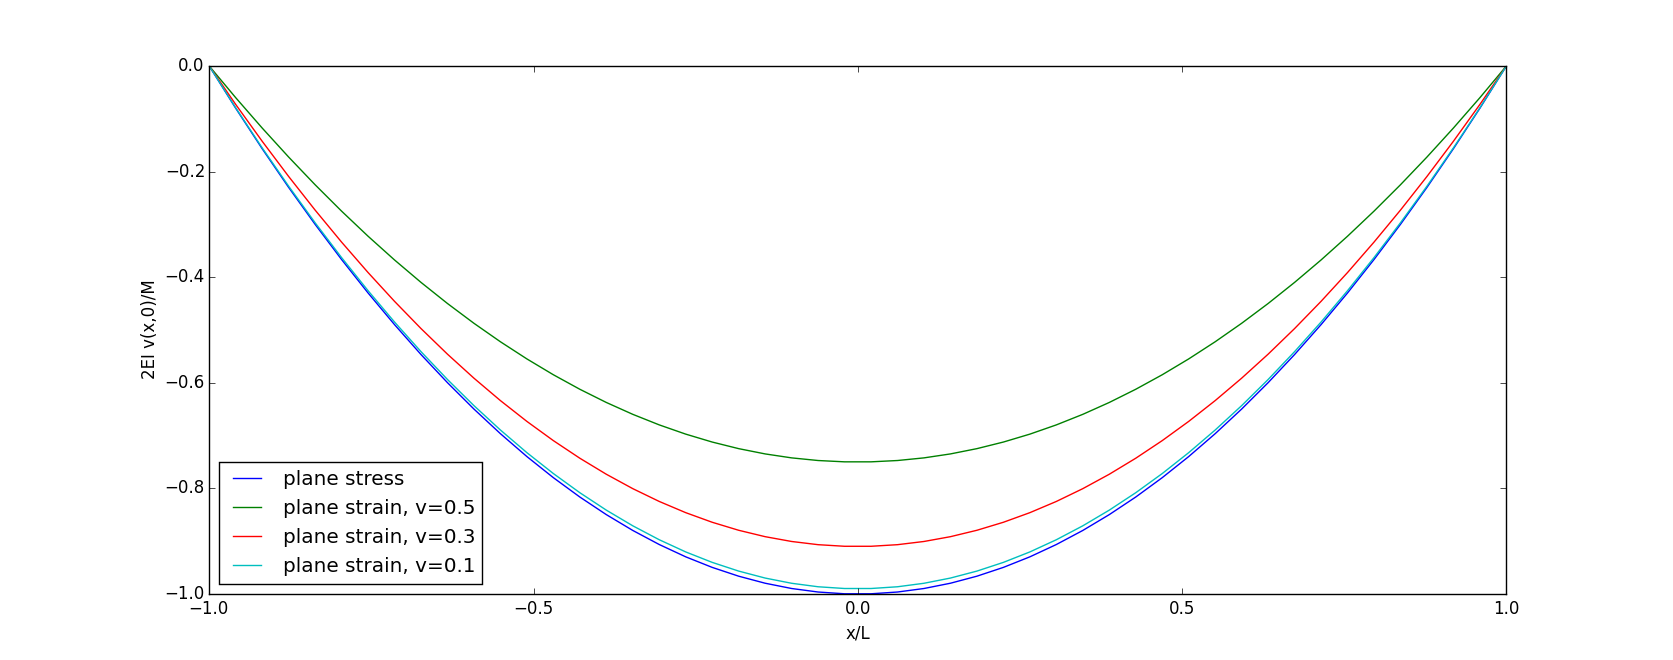
\includegraphics{../images/figure_1.png}
\caption{beam bending example}
\end{figure}
\end{frame}

\end{document}
